\partstart{Thử nghiệm và kết quả}
\subsection{Môi trường, dữ liệu và cấu hình thực nghiệm}
Số liệu phần này lấy từ các bảng và hình công bố trong \code{results}.
Manifest ghi SHA256 nguồn, encoding CP1252 và protocol lấy mẫu nhóm.
Tập kiểm tra là holdout lịch sử đã được quan sát
trong quá trình phát triển; việc biên tập và đối chiếu báo cáo không tạo
ra một lần đánh giá độc lập mới.

\begin{table}[!htbp]\centering
\caption{Quy mô thực tế của nguồn, mẫu và các tập sau split.}\label{tab:split}
\begin{tabularx}{\linewidth}{Yrr}\toprule
\theadcell{Phạm vi} & \theadcell{Số dòng} & \theadcell{Số đơn}\\\midrule
Toàn nguồn & 180.519 & 65.752\\
Mẫu thực nghiệm & 5.999 & 2.113\\
Huấn luyện & 4.823 & 1.690\\
Kiểm tra & 1.176 & 423\\\bottomrule
\end{tabularx}

\end{table}
Theo Bảng~\ref{tab:split}, mẫu chỉ chiếm 3,32\% số dòng và 3,21\% số đơn
nguồn. Giới hạn này được đặt để kiểm soát tài nguyên cho K-NN và tìm kiếm
tham số. Không gọi đây là kết quả huấn luyện trên toàn bộ DataCo. Số dòng
trung bình mỗi đơn là 2,839 trong mẫu và 2,745 trong toàn nguồn; kích thước
đơn tối đa ở cả hai là năm dòng.

Cấu hình seed 42, ba fold nhóm và một tiến trình được giữ chung cho sáu
ứng viên. Môi trường phiên bản lấy từ manifest đã trình bày ở Chương~\ref{chap:3};
manifest không ghi đủ CPU/RAM để đưa ra kết luận benchmark phần cứng.
Thời gian được lưu là thời gian đo của lần chạy, không phải cam kết độ
trễ của dịch vụ triển khai. Tất cả mô hình dùng cùng split và cùng fold.

\subsection{Bảng kết quả chung và tiêu chí lựa chọn}
\begin{table}[!htbp]\centering\small
\begin{tabular}{lrrrrr}\toprule
Mô hình & CV F1 & Accuracy & Precision & Recall & F1 \\\midrule
baseline\_tree\_A & 0.6691 & 0.6531 & 0.6986 & 0.6234 & 0.6589 \\
dummy\_A & 0.6944 & 0.5374 & 0.5374 & 1.0000 & 0.6991 \\
knn\_A & 0.6668 & 0.6735 & 0.7230 & 0.6361 & 0.6768 \\
tree\_A & 0.6741 & 0.6463 & 0.6731 & 0.6646 & 0.6688 \\
knn\_B & 0.6714 & 0.6862 & 0.7295 & 0.6614 & 0.6938 \\
tree\_B & 0.7058 & 0.7330 & 0.8533 & 0.6076 & 0.7098 \\
\bottomrule\end{tabular}
\caption{Metric theo dòng; CV trên train, bốn cột cuối trên test lịch sử.}\label{tab:metrics}
\end{table}

Bảng~\ref{tab:metrics} giữ bốn thước đo test và điểm CV F1. Tree B có CV F1
cao nhất 0,7058, hơn Dummy khoảng 0,0114. Theo protocol đã định, nó được
khóa là mô hình chọn trước khi xem test. Trên test, tree B đạt Accuracy
0,7330, Precision 0,8533, Recall 0,6076 và F1 0,7098. Không dùng tên
``tốt nhất'' để suy rộng ra mọi thước đo: Dummy có Recall cao hơn và K-NN B
có Recall cao hơn cây B.

\fig[.96]{comparison.png}{So sánh điểm CV và các metric test của sáu ứng viên.}{fig:comparison}
Hình~\ref{fig:comparison} làm rõ các cấu hình có hướng đánh đổi khác nhau.
Cây B nổi bật ở Precision nhưng không dẫn đầu Recall. F1 của Dummy tương
đối cạnh tranh dù mô hình không phân biệt từng đơn. Vì vậy, các cột metric
cần được đọc cùng nhau; chỉ nhìn F1 hoặc chỉ nhìn Accuracy sẽ bỏ qua số
đơn trễ bị bỏ sót và mức tải cảnh báo.

Chênh lệch F1 test giữa cây B và Dummy khoảng 0,0107, chưa có khoảng tin
cậy cho chênh lệch này. Ba fold CV là quá ít để khẳng định một cách ổn định
rằng mô hình thắng luôn vượt đối chứng. Báo cáo giữ kết quả theo quy tắc
lựa chọn ban đầu, đồng thời trình bày đầy đủ các đối chứng để người đọc
đánh giá mức cải thiện thực tế.

\subsection{Dummy và cây quyết định baseline}
Dummy most-frequent luôn dự đoán 1 trong lần chạy này. Trên test, nó tạo
632 TP, 544 FP, không có TN hoặc FN. Accuracy và Precision đều bằng
$632/1176=0{,}5374$, Recall bằng 1 và F1 bằng 0,6991. Điểm cao này xuất
phát từ tỷ lệ lớp dương và cách F1 thưởng cho Recall, không thể hiện khả
năng xếp ưu tiên các đơn cần kiểm tra.

\fig[.65]{dummy_A_confusion.png}{Ma trận nhầm lẫn của Dummy A trên 1.176 dòng test.}{fig:cm-dummy}
Trong Hình~\ref{fig:cm-dummy}, cột dự đoán 0 bằng 0 ở cả hai lớp thật.
Nếu sử dụng quy tắc này làm cảnh báo, mọi dòng đều cần xử lý. Đây là mốc
so sánh minh bạch: cây B giảm mạnh cảnh báo sai nhưng chấp nhận bỏ sót.
Không xem ``không bỏ sót'' là đủ để xác nhận hữu ích vận hành khi nguồn lực
đánh giá cảnh báo có giới hạn.

Cây baseline đạt F1 train 0,9994 nhưng CV chỉ 0,6691, test F1 0,6589.
Khoảng cách train--CV 0,3303 là dấu hiệu mô hình khớp rất mạnh dữ liệu
học nhưng không giữ cùng hiệu quả ở đơn chưa thấy. Nó dùng lá tối thiểu
1 và không giới hạn độ sâu, phù hợp với diễn giải về độ phức tạp cao.
Tuy nhiên, đây là dấu hiệu mô tả, không phải phép thử nhân quả riêng cho
từng siêu tham số.

\fig[.65]{baseline_tree_A_confusion.png}{Ma trận nhầm lẫn của cây mặc định với luồng A.}{fig:cm-base}
Hình~\ref{fig:cm-base} cần được đọc cùng F1 train gần hoàn hảo. Một kết
quả train cao không bảo đảm mô hình phát hiện tốt trên test. Precision
0,6986 và Recall 0,6234 của baseline đều thấp hơn mức cần thiết để kết
luận ứng dụng mà không có tiêu chí nghiệp vụ; baseline chủ yếu giúp thấy
giá trị của việc kiểm soát độ phức tạp và lựa chọn mô hình có hệ thống.

\subsection{K-NN với hai luồng đặc trưng}
Cả K-NN A và B được chọn với 15 láng giềng, trọng số distance và khoảng
cách Euclidean trong lưới đã thử. K-NN A có CV F1 0,6668, test F1 0,6768;
K-NN B có CV F1 0,6714, test F1 0,6938. Test Precision tăng từ 0,7230 lên
0,7295 và Recall tăng từ 0,6361 lên 0,6614. Đây là thay đổi quan sát được
khi bổ sung lịch trên cùng protocol.

\begin{figure}[!htbp]\centering
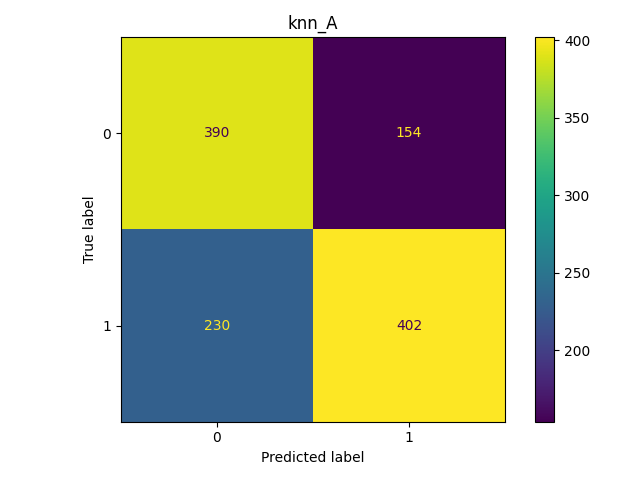
\includegraphics[width=.47\textwidth]{../results/figures/knn_A_confusion.png}\hfill
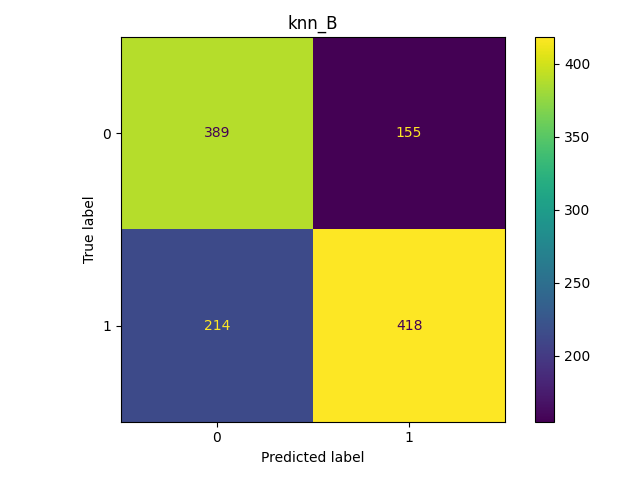
\includegraphics[width=.47\textwidth]{../results/figures/knn_B_confusion.png}
\caption{Ma trận nhầm lẫn K-NN: A bên trái và B bên phải.}\label{fig:cm-knn}
\end{figure}
Từ Hình~\ref{fig:cm-knn} và bảng số đếm, A có TN=390, FP=154, FN=230,
TP=402; B có TN=389, FP=155, FN=214, TP=418. B phát hiện thêm 16 dòng
dương nhưng tăng một FP trong tổng hợp. Những số đếm này không cho biết
đó có phải cùng các đơn hay không và không nên coi 16 dòng là 16 trường
hợp độc lập do cấu trúc nhiều mặt hàng trong đơn.

F1 train của A là 0,9994 và B là 1,0000. Khoảng cách train--CV lần lượt
0,3326 và 0,3286 rất lớn. Với trọng số distance, dự đoán trên chính các
điểm train có thể bị chi phối bởi điểm cách 0, nên F1 train cao của K-NN
không phải thước đo thuyết phục về tổng quát hóa. CV theo nhóm mới tạo
tình huống đơn chưa xuất hiện trong phần học của fold.

\subsection{Cây quyết định với A và B}
Cây A được chọn với gini, không giới hạn độ sâu và tối thiểu 20 mẫu/lá.
CV F1 là 0,6741, test F1 0,6688. Cây B cũng dùng gini và tối thiểu 20
mẫu/lá nhưng độ sâu tối đa 4; CV F1 đạt 0,7058 và test F1 0,7098.
So với A, B tăng CV F1 khoảng 0,0316 và test F1 khoảng 0,0410, đồng thời
đánh đổi Recall lấy Precision.

\begin{figure}[!htbp]\centering
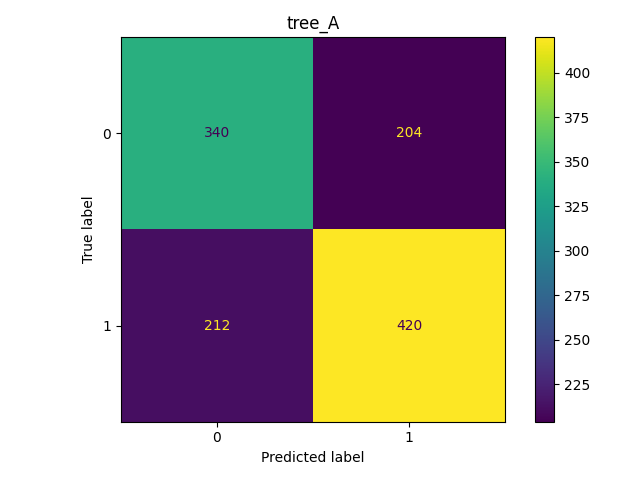
\includegraphics[width=.47\textwidth]{../results/figures/tree_A_confusion.png}\hfill
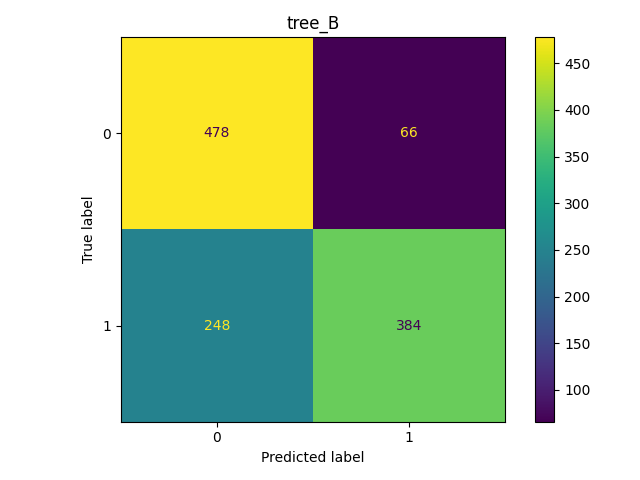
\includegraphics[width=.47\textwidth]{../results/figures/tree_B_confusion.png}
\caption{Ma trận nhầm lẫn cây A (trái) và cây B được chọn theo CV (phải).}\label{fig:cm-tree}
\end{figure}
Hình~\ref{fig:cm-tree} cho thấy cây A có TN=340, FP=204, FN=212, TP=420. Cây B có TN=478, FP=66, FN=248,
TP=384. Vì vậy, B giảm 138 FP nhưng tăng 36 FN so với A. Từ số đếm này,
không thể kết luận tổng chi phí giảm khi chưa biết giá của một cảnh báo
sai và một bỏ sót. Đây là ví dụ cụ thể cho thấy F1 cao hơn không đồng
nghĩa mọi loại lỗi đều ít hơn.

\begin{samepage}
Theo định nghĩa từ Chương~\ref{chap:2}, kiểm tra lại cây B cho
$P=384/(384+66)=0{,}8533$ và $R=384/(384+248)=0{,}6076$.
Công thức F1 theo số đếm cho $768/(768+66+248)=0{,}7098$.
Như vậy, metric trong bảng phù hợp trực tiếp với ma trận nhầm lẫn, không
lấy từ con số làm tròn trên ảnh. ROC-AUC là 0,7756 và average precision
là 0,7889; hai chỉ số không xác nhận xác suất đã hiệu chuẩn.
\par\end{samepage}

\subsection{Cross-validation, dao động và overfitting}
\begin{table}[!htbp]\centering
\caption{Mức khớp trên train, CV và chênh lệch F1 của sáu ứng viên.}\label{tab:gaps}
\begin{tabularx}{\linewidth}{Ycrrrr}\toprule
\rowcolor{reportheader} \theadcell{Mô hình} & \theadcell{Luồng} & \theadcell{Train F1} & \theadcell{CV F1} & \theadcell{SD CV} & \theadcell{Train--CV} \\\midrule
Cây cơ sở & A & 0.9994 & 0.6691 & 0.0138 & 0.3303 \\
Dummy & A & 0.6944 & 0.6944 & 0.0001 & -0.0000 \\
K-NN & A & 0.9994 & 0.6668 & 0.0060 & 0.3326 \\
Cây & A & 0.7646 & 0.6741 & 0.0154 & 0.0905 \\
K-NN & B & 1.0000 & 0.6714 & 0.0161 & 0.3286 \\
Cây & B & 0.7137 & 0.7058 & 0.0102 & 0.0079 \\
\bottomrule\end{tabularx}
\end{table}

Trong Bảng~\ref{tab:gaps}, cây B có chênh lệch train--CV nhỏ nhất trong các
mô hình dùng đặc trưng, khoảng 0,0079. Đây là dấu hiệu khả quan về mức
khớp trong protocol hiện tại. Tuy nhiên, khoảng cách nhỏ cũng có thể đi
cùng mô hình còn đơn giản và bỏ sót một nhóm lớn; kết quả Standard Class
bên dưới cho thấy không được dùng gap nhỏ để khẳng định mô hình đã đủ tốt.

Độ lệch chuẩn CV F1 của K-NN A khoảng 0,0060, K-NN B 0,0161, cây A
0,0154 và cây B 0,0102. Không gán ý nghĩa thống kê cho việc chênh lệch
trung bình lớn hay nhỏ hơn một độ lệch chuẩn. Cần repeated group split
hoặc đánh giá độc lập có thiết kế trước để đo độ ổn định. Điểm test nhỉnh
hơn CV ở một số ứng viên có thể phản ánh khác biệt độ khó của tập dữ liệu;
không chứng minh test bị dùng để huấn luyện.

Thời gian search/refit ghi nhận khoảng 41,70 giây cho K-NN A, 39,34 giây
cho K-NN B, 13,18 giây cho cây A và 19,09 giây cho cây B. Đây là chi phí
của các lưới có số cấu hình khác nhau trên một máy ở lần chạy lịch sử.
Không so sánh như benchmark tốc độ thuật toán độc lập và không suy ra
độ trễ cho từng đơn khi triển khai.

\subsection{EDA: giá trị thiếu và đặc trưng số}
\fig[.78]{02_missing.png}{Tỷ lệ thiếu trên train; chỉ thể hiện các cột thiếu nhiều nhất.}{fig:missing}
Hình~\ref{fig:missing} phản ánh cột mô tả sản phẩm thiếu hoàn toàn và mã
bưu chính đơn thiếu rất nhiều. Đây là những cột không được phép đi vào
pipeline. Hình không chứng minh rằng đầu vào mô hình đang thiếu ở mức
tương tự; Bảng~\ref{tab:missing} mô tả toàn nguồn còn hình chỉ mô tả train.
Không dùng mức thiếu ở cột bị loại để giải thích chênh lệch A/B.

\fig[.88]{03_numeric_hist.png}{Histogram bốn đặc trưng số trên train, trước scaling.}{fig:hist}
Hình~\ref{fig:hist} giúp nhận diện thang đo khác nhau giữa số ngày, số
lượng, giá và tỷ lệ chiết khấu. Những đỉnh của biến rời rạc không mặc
nhiên là bất thường; ví dụ số ngày kế hoạch và số lượng vốn có miền giá
trị hạn chế. Giá sản phẩm cần được xem xét ở thang riêng trước khi tính
khoảng cách. Đây là căn cứ phương pháp cho chuẩn hóa, chưa là thí nghiệm
chứng minh chuẩn hóa tăng bao nhiêu F1.

\fig[.78]{04_boxplot.png}{Boxplot đặc trưng số trên train với thang giá trị gốc.}{fig:box}
Do các trường chung trục gốc, trường giá có thể chiếm phần lớn chiều dài
Hình~\ref{fig:box}. Không suy ra các trường còn lại không biến thiên chỉ
vì chúng nhìn hẹp trên hình này. Báo cáo kết hợp histogram riêng và thống
kê số để tránh đọc sai tác động của thang đo. Không cắt bỏ các điểm được
đánh dấu IQR; pipeline hiện tại không có bước clipping hoặc winsorization.

\subsection{EDA: phương thức giao hàng và khu vực}
\fig[.76]{05_shipping.png}{Số dòng từng lớp theo phương thức giao hàng trên train.}{fig:shipping}
Hình~\ref{fig:shipping} đặt số đếm hai lớp cạnh nhau theo phương thức
giao. Đây là cấu trúc đáng chú ý vì cây B sau đó phân nhánh mạnh theo
Shipping Mode. Tuy nhiên, từ countplot không thể kết luận chọn phương
thức giao nhanh gây trễ: thời hạn cam kết, loại đơn và phân khúc khách
có thể khác nhau đồng thời. Cần giữ tách biệt mô tả mối liên hệ với kết
luận nhân quả.

\fig[.82]{06_regions.png}{Tỷ lệ dòng trễ theo vùng trên train, không phải số lượng đơn.}{fig:regions}
Hình~\ref{fig:regions} được đọc cùng \code{train_region_support.csv}.
Central America có 767 dòng với tỷ lệ trễ 0,5306; Western Europe 614 dòng
với 0,5326. Central Asia có tỷ lệ 0,8261 nhưng chỉ 23 dòng, trong khi
Canada có 10 dòng. Cột cao của một vùng ít quan sát không cung cấp độ
chắc chắn tương đương vùng nhiều quan sát, và các dòng còn phụ thuộc theo
đơn. Không xếp hạng chất lượng vận hành các vùng chỉ bằng hình này.

\subsection{EDA: tương quan và diễn biến theo tháng}
\fig[.73]{07_correlation.png}{Tương quan tuyến tính giữa bốn trường số trên train.}{fig:corr}
Hình~\ref{fig:corr} khảo sát quan hệ từng cặp giữa các đầu vào số, không
phải độ quan trọng mô hình. Tương quan thấp không loại trừ quan hệ phi
tuyến hoặc tương tác với phương thức giao. Ngược lại, tương quan cao
giữa hai trường cũng không tự tạo leakage nếu cả hai có sẵn ở thời điểm
dự đoán. Quyết định loại trường phải kết hợp thời điểm, ngữ nghĩa và
thiết kế thí nghiệm, không chỉ dựa hệ số tương quan.

\fig[.96]{08_month.png}{Tỷ lệ trễ theo tháng tạo đơn trên train, ghép năm--tháng.}{fig:month}
Hình~\ref{fig:month} là đường mô tả theo các khoảng năm--tháng, trong khi
đặc trưng \code{order_month} chỉ lấy tháng trong năm. Không đồng nhất hai
cách biểu diễn. Dao động trên hình gợi ý cần kiểm tra cấu trúc thời gian,
nhưng chưa chứng minh mùa vụ ổn định; số đơn mỗi tháng và thay đổi cơ cấu
đơn có thể ảnh hưởng tỷ lệ. Split nhóm ngẫu nhiên không kiểm tra khả năng
dự đoán những tháng nằm sau giai đoạn train.

\subsection{Đánh giá theo đơn và độ nhạy với đơn vị quan sát}
\begin{table}[!htbp]\centering\small
\caption{Metric theo đơn, xác suất trung bình và ngưỡng 0,5 cố định.}\label{tab:orders}
\begin{tabular}{lrrrr}\toprule
Mô hình & Accuracy & Precision & Recall & F1 \\\midrule
tree\_B & 0.7258 & 0.8554 & 0.6068 & 0.7100 \\
dummy\_A & 0.5532 & 0.5532 & 1.0000 & 0.7123 \\
\bottomrule\end{tabular}
\end{table}

Bảng~\ref{tab:orders} lấy xác suất trung bình theo 423 đơn và ngưỡng 0,5.
Tree B có TN=165, FP=24, FN=92, TP=142; Dummy có TN=0, FP=189, FN=0,
TP=234. F1 cây B theo đơn là 0,7100, gần F1 dòng 0,7098, nhưng Dummy
đạt 0,7123 và nhỉnh hơn cây B ở cấp đơn. Vì vậy, thứ tự theo F1 test có
thể phụ thuộc đơn vị tính, ngay cả khi split không đổi.

Điểm theo đơn không được dùng để chọn lại mô hình sau khi xem holdout.
Nó là chẩn đoán bổ sung về tính phù hợp với nghiệp vụ. Đơn nhiều dòng
được trọng số lớn trong metric dòng; metric đơn khắc phục cách đếm đó
nhưng cần quy tắc tổng hợp xác suất. Chưa kiểm tra quy tắc max hoặc các
ngưỡng khác; không tuyên bố trung bình là lựa chọn tối ưu.

\subsection{Ablation thời gian và phân tích lỗi theo nhóm}
\begin{table}[!htbp]\centering\small
\begin{tabular}{lrrr}\toprule
Thuật toán & A: CV F1 & B: CV F1 & B--A \\\midrule
knn & 0.6668 & 0.6714 & +0.0046 \\
tree & 0.6741 & 0.6904 & +0.0163 \\
\bottomrule\end{tabular}
\caption{Ablation lịch trên CV train với tham số của A được giữ cố định.}\label{tab:ablation}
\end{table}

Trong Bảng~\ref{tab:ablation}, cấu hình của A được cố định khi thay luồng.
K-NN tăng CV F1 khoảng 0,0046; cây tăng khoảng 0,0163. Kết quả khác với
mức tăng 0,0316 khi mỗi luồng cây tự chọn tham số riêng. Điều này cho
thấy so sánh tuned A/B trộn cả thay đổi đặc trưng lẫn lựa chọn siêu tham
số. Ablation giúp tách bớt hai yếu tố, nhưng vẫn đánh giá trên fold đã
dùng chọn tham số A nên chưa loại selection optimism.

\begin{table}[!htbp]\centering
\caption{Lỗi theo dòng của cây B, kèm mẫu số nhóm dịch vụ.}\label{tab:shipping-errors}
\begin{tabularx}{\linewidth}{Yrrrrrr}\toprule
\theadcell{Phương thức} & \theadcell{n} & \theadcell{Dương} & \theadcell{FN} & \theadcell{FP} & \theadcell{FNR} & \theadcell{FPR} \\\midrule
First Class & 203 & 193 & 0 & 10 & 0.0000 & 1.0000 \\
Same Day & 71 & 27 & 0 & 0 & 0.0000 & 0.0000 \\
Second Class & 198 & 158 & 0 & 40 & 0.0000 & 1.0000 \\
Standard Class & 704 & 254 & 248 & 16 & 0.9764 & 0.0356 \\
\bottomrule\end{tabularx}
\end{table}

\begin{samepage}
Bảng~\ref{tab:shipping-errors} ghi toàn bộ 248 FN ở Standard Class: sáu TP
trên 254 dòng dương (Recall 0,0236), 16 FP trên 450 dòng âm. First Class
có 10 FP/10 dòng âm, Second Class 40 FP/40 dòng âm. Same Day không lỗi
trên 71 dòng, chưa đủ khẳng định ổn định. Các lỗi nhóm là chẩn đoán,
không dùng để tinh chỉnh lại trên test; Chương~\ref{chap:5} phân tích giới hạn này.
\par\end{samepage}
